% !TeX root = RJwrapper.tex
\title{dapper: An R Package for studying differentially private algorithms}


\author{by Jordan A. Awan, Kevin Eng, Robin Gong, Nianqiao Phyllis Ju, and Vinayak A. Rao}

\maketitle

\abstract{%
This paper serves as a reference and introduction on using the dapper R package. The goal of this package is to provide some tools for exploring the impact of different privacy regimes on a Bayesian analysis. A strength of this framework is the ability to target the exact posterior in settings where the likelihood is too complex to analytically express.
}

\hypertarget{introduction}{%
\section{Introduction}\label{introduction}}

Differential privacy provides a rigorous framework for protecting
confidential information. One of it's goal is to allow the widespread dissemination
of summary statistics while hiding sensitive characteristics of the data.
For example, a data aggregation service might
collect salary information for the purpose of helping its users negotiate salaries.
Such information is typically considered both sensitive. In this scenario, there is a strong desire
to simultaneously keep the salary information of individuals anonymous and make
queries of the salary database publicly available.

In the context of statistical models,
considerable effort has been put in ensuring privacy is
achieved by using two methods. The first method consist of first fitting the model to the
confidential data set and then adding noise to its output. The second method
injects noise at some point in the model fitting process. The fitting process in many models can be
viewed as minimizing a loss function. Privacy can be achieved by
adding random perturbations to the loss function. See (Ji, Lipton, and Elkan 2014) for a
survey that covers the two methods applied to variety of commonly used
machine learning models. On the other hand, adding noise directly to the data is a less
studied approach and is the case which this paper addresses.

Statistical regression models typically assume no measurement error in the observed covariate data.
In the presence of such errors, standard estimators can exhibit significant bias (Gong 2022).
Therefore, fitting standard statistical models after adding noise directly to the data for privacy can lead to incorrect
inference. Adjusting models to take into account noisy covariates has a rich history
spanning several decades. For textbook length treatments see (Yi 2017; Carroll et al. 2006).
Prior work mostly focuses on methods which did not require fully specifying the
measurement error model, since this was often unknown.
However, in differential privacy, the measurement error model is exactly known.
This difference, makes feasible some ideas which the measurement
error community has not previously considered (Smith 2011; Karwa, Kifer, and Slavković 2015).

One approach, to account for the added noise, is to treat the confidential data
as latent quantities within a statistical model. In such settings, it is common
to conduct inference by specifying a complete likelihood. Once the complete likelihood
has been specified, parameter estimation can be done using the EM algorithm or
its Bayesian analogue, the data augmentation method. In the case of dapper,
inference is done using data augmentation as described in (Ju et al. 2022). A notable benefit of the Bayesian
approach is that both uncertainty quantification and estimation are done
simultaneously. The EM approach only provides an estimate.

The rest of this article is organized as follows. Section 2 covers the necessary background to understand the mathematical notation
and ideas used throughout the paper. Section 3 goes over the main algorithm without
going into mathematical detail, for specifics see (Ju et al. 2022). Section 4 provides
an overview of the dapper package and discusses important implementation details.
Section 5 contains two example of how one might use the package to analyze the
impact of adding noise for privacy.

\hypertarget{background}{%
\section{Background}\label{background}}

Let \(x = (x_1, \ldots, x_n) \in \mathcal{X}^n\) represent a confidential
database containing \(n\) records. Usually the goal of collecting data
is to learn some characteristic about the underlying population.
To accomplish this task, a common approach is to assume the population
is represented by some statistical model \(f( \cdot \mid \theta)\). It is often the case that
some function of \(\theta\) has relevant meaning to the scientific question at hand. In this setting,
learning characteristics of a population reduces to learning about \(\theta\).

In the Bayesian framework, this is accomplished by drawing samples from the
posterior \(p(\theta \mid x) \propto f(x \mid \theta) p(\theta)\). For
large data sets, it is common to work with a summary statistic \(s = s(x)\)
that has much smaller dimension than the original data. Doing so can
greatly simplify calculations. In general, there can be information
loss with using summary statistics, but for models with a sufficient
statistic, there is no loss. In the context of privacy, providing
a summary statistic can offer a level of anonymity.

\hypertarget{differential-privacy}{%
\subsection{Differential Privacy}\label{differential-privacy}}

While a summary statistic can already anonymize the data, it is still
possible to deduce information about an individual entry depending on
the distribution of \(x\). For additional anonymity, one idea is to
add noise to the summary statistic \(s\). More formally we write
\(s_{dp} \sim \eta(\cdot \mid x)\). Here, \(s_{dp}\) is the noise infused version of \(s\) and
\(\eta\) is a known noise infusion process. The privacy mechanism
\(\eta\) is said to be \(\epsilon\)-differentially private (Dwork and Roth 2013) if for all values of
\(s_{dp}\), and all ``neighboring'' databases \((x,x') \in \mathcal{X}^n \times \mathcal{X}^n\) differing
by one record (denoated by \(d(x,x')\)), the probability ratio is bounded:
\[
\dfrac{\eta(s_{dp} \mid x)}{\eta(s_{dp} \mid x')} \leq \exp(\epsilon), \quad \epsilon > 0.
\]
The parameter \(\epsilon\) is called the privacy loss budget, and controls how informative \(s_{dp}\)
is about \(x\). Larger values of \(\epsilon\) correspond to less noise being added.

\hypertarget{data-augmentation}{%
\subsection{Data Augmentation}\label{data-augmentation}}

The idea behind data augmentation is to run a Gibbs sampler on a coupling of two random variables where one
of the marginals is the target distribution. Suppose we wish to sample from a density \(f_{A}\) which is difficult.
The data augmentation method instead considers sampling from a joint distribution \(f(a,b)\). Since
we are ultimately interested in samples from \(f_A\), the joint
distribution should be chosen so that (i) the marginal distribution
with respects to \(a\) is \(f_{A}\) and (ii) \(f(a \mid b)\) and \(f(b \mid a)\)
are easy to sample from. The choice \(f\) is not unique and can require
some foresight.

\hypertarget{methodology}{%
\section{Methodology}\label{methodology}}

Given data \(s_{dp}\), the goal of Bayesian inference is to sample from the
posterior distribution \(p(\theta \mid s_{dp})\). Since the observed likelihood,
\(p(s_{dp} \mid \theta)\) often has no simple closed form expression, most standard
sampling schemes do not apply. To conduct privacy aware Bayesian inference, the dapper package implements
the data augmentation algorithm which allows us to sample from \(p(\theta \mid s_{dp})\)
without needing to specify \(p(s_{dp} \mid \theta)\).

The algorithm considers the joint distribution \(p(\theta, x \mid s_{dp})\) and
alternates sampling from the two distributions

\begin{itemize}
\tightlist
\item
  \(p(\theta \mid x, s_{dp})\)
\item
  \(p(x \mid \theta, s_{dp})\)
\end{itemize}

Since \(s_{dp}\) is derived from \(x\), we have \(p(\theta \mid x, s_{dp}) = p(\theta \mid x)\) which
is just the usual posterior distribution given the confidential data \(x\). The dapper
package assumes the user has access to a sampler for \(p(\theta \mid x)\). This can
come from any R package such as fmcmc. For the second distribution, \(p(x \mid \theta, s_{dp})\), may
only be known up to a constant. The dapper package samples from this distribution by
running a Gibbs like sampler. Each of the \(n\) components of \(x\) is individually
updated. However unlike the standard Gibbs sampler, each component is updated
using a Metropolis-Hasting algorithm. This method is sometimes called the Metropolis within Gibbs sampler (Robert and Casella 2004).

In some cases, sampling from \(p(x \mid \theta, s_{dp})\) can be made more efficient
when the summary statistic can be written as the sum of individual
contributions from each observation. More precisely, we say a statistic satisfies
the record additivity property if \(\eta(s_{dp} \mid x) = g(s_{dp}, \sum_{i=1}^{n}t_i(x_i, s_{dp}))\)
for some known and tractable functions \(g, t_1, \ldots, t_n\).

The algorithm is in the following pseudo code:

\begin{enumerate}
\def\labelenumi{\arabic{enumi}.}
\tightlist
\item
  Sample \(\theta^{t+1}\) from \(p(\cdot \mid x^{(t)})\).
\item
  Sample from \(p(x \mid \theta, s_{dp})\) using a three step process

  \begin{itemize}
  \tightlist
  \item
    Propose \(x_{i}^{*} \sim f(\cdot \mid \theta)\).
  \item
    If \(s\) satisfies the record additive property then
    update \(s(x^*, s_{dp}) = t(x,s_{dp}) - t_i(x_i,s_{dp}) + t_{i}(x_i^*, s_{dp})\).
  \item
    Accept the proposed state with probability \(\alpha(x_i^* \mid x_i, x_{-i}, \theta)\)
    given by:
  \end{itemize}

  \[
     \alpha(x_i^* \mid x_i, x_{-i}, \theta) = \min \left\{ \dfrac{\eta(s_{dp} \mid x_i^*, x_{-i})}{\eta(s_{dp} \mid x_i, x_{-i})} \right\}.
   \]
\end{enumerate}

\hypertarget{using-dapper}{%
\section{Using dapper}\label{using-dapper}}

The package is structured around the two functions \texttt{dapper\_sample} and
\texttt{new\_privacy}. The first function is used to draw samples from the
posterior. The second function is used to create the privacy model. Since the
input to these functions are R functions, there is a great deal of freedom
left up to user. The next two sections describe in detail the inputs into
these functions and highlight some considerations that should be taken
into account in order avoid slow or unexpected behavior.

Before delving into the specifics of each component, it is necessary to clearly
define how the confidential data is represented. Internally, the
confidential database is encoded as a 2D matrix. There are often multiple ways
of doing this. For example, if our data consist
of 100 responses from a two question, yes/no, survey. Then we can either encode
the data as a \(2 \times 2\) matrix, or a \(100 \times 2\) matrix. Both are mathematically
equivalent, but the \(2 \times 2\) matrix will be much more memory efficient.
In general, the representation that uses the least amount of memory should be
used. Correctly specifying the privacy model will require a consistent
representation among all components.

\hypertarget{sampling}{%
\subsection{Sampling}\label{sampling}}

The main function in \pkg{dapper} is the \texttt{gdp\_sample} function. The call
signature of the function is:

\begin{verbatim}
gdp_sample(data_model, sdp, nobs, init_par, niter = 2000, warmup = floor(niter / 2),
           chains = 1, varnames = NULL)
\end{verbatim}

The three required inputs into \texttt{gdp\_sample} function are the privacy model (\texttt{data\_model}), the value
of the observed privatized statistic (\texttt{sdp}), and the total number of observations
in the complete data (\texttt{nobs}). The dapper
package is best suited for problems where the complete data can be represented in
tabular form. This is because internally, it is represented as a matrix.

The optional arguments are the number of mcmc draws (\texttt{niter}), the
burn in period (\texttt{warmup}), number of chains (\texttt{chains}) and character
vector that names the parameters. Running multiple chains can be done in parallel
using the \CRANpkg{furrr} package. Additionally, progress can be monitored
using the \CRANpkg{progressr} package.

The \texttt{data\_model} input is a \texttt{privacy}
object that can be constructed using the \texttt{new\_privacy} constructor. The
process of constructing a \texttt{privacy} object will be discussed in the next section.

\hypertarget{privacy-model}{%
\subsection{Privacy Model}\label{privacy-model}}

Creating a privacy model is done using the \texttt{new\_privacy} constructor. The
main arguments consist of the four components as outlined in the methodology
section.

\begin{verbatim}
new_privacy(post_smpl = NULL, lik_smpl = NULL, ll_priv_mech = NULL,
            st_calc = NULL, add = FALSE, npar = NULL)
\end{verbatim}

The internal implementation of the DA algorithm in \texttt{dapper\_sample} requires
some care in how each component is constructed.

\begin{itemize}
\item
  \texttt{lik\_smpl} is an R function that samples from the likelihood. Its
  call signature should be \texttt{lik\_smpl(theta)} where \texttt{theta} is a vector
  representing the likelihood model parameters being estimated. This function
  must work with the supplied initial parameter provide in the \texttt{init\_par}
  argument of \texttt{dapper\_sample} function and its output should be a \(n \times k\) matrix. \(k\) the
  dimension of the complete data table.
\item
  \texttt{post\_smpl} is a function which represents the posterior sampler. It should
  have the call signature \texttt{post\_smpl(dmat,\ theta)}. Where \texttt{dmat} is the
  complete data. This sampler can be generated by wrapping mcmc samplers generated from other R packages
  (e.g.~\CRANpkg{rstan}, \CRANpkg{fmcmc}, \CRANpkg{adaptMCMC}).
  If using this approach, it is recommended to avoid using packages such as \CRANpkg{mcmc}
  whose implementation clashes with \texttt{gdp\_sample}. In the case of \CRANpkg{mcmc},
  the Metropolis-Hastings loop is implemented in C which incurs a very large overhead
  in \texttt{gdp\_sample} since it is reinitialized every iteration. In general, repeatedly calling
  an R function that hooks into C code is slow. (NOT QUITE ACCURATE FIX LATER)
\item
  \texttt{ll\_priv\_mech} is an R function that represents the log-likelihood of
  \(\eta(s_{sdp} \mid x)\). The function can output the log likelihood
  up to an additive constant.
\item
  \texttt{st\_calc} is an R function which calculates the summary statistic. The optional
  argument \texttt{add} is a flag which represents whether \(T\) is additive or not.
\end{itemize}

\hypertarget{examples}{%
\section{Examples}\label{examples}}

\hypertarget{x2-contingency-table}{%
\subsection{2x2 Contingency Table}\label{x2-contingency-table}}

A common procedure when analyzing contingency tables is to estimate the
odds ratio. Something something about safetab to connect back to DP (dont forget citation!).
As a demonstration, we analyze the UC Berkeley admissions data, which is often
used as an illustrative example of Simpson's paradox. The question is whether
the data suggest there is bias against females during the college admissions
process. Below is a table of the aggregate admissions result from six departments based on sex.

\begin{table}[!h]

\centering
\begin{tabular}[t]{lrr}
\toprule
  & Male & Female\\
\midrule
Admitted & 1198 & 557\\
Rejected & 1493 & 1278\\
\bottomrule
\end{tabular}
\centering
\begin{tabular}[t]{lrr}
\toprule
  & Male & Female\\
\midrule
Admitted & 1135 & 473\\
Rejected & 1511 & 1438\\
\bottomrule
\end{tabular}
\end{table}

Below we walk through the process of defining a privacy model.

\begin{enumerate}
\def\labelenumi{\arabic{enumi}.}
\item
  \texttt{lik\_smpl}: Conditional on the table total, the table counts follow a multinomial
  distribution. We can easily draw from this distribution using the
  \texttt{rmultinom} function in the \texttt{base} stats package. Note, in this example,
  the return value of one sample from \texttt{rmultinom} is a \(4 \times 1\) matrix. In order to
  conform with \texttt{dapper\_sample} we must convert the matrix to a vector.

\begin{verbatim}
lik_smpl <- function(theta) {
  t(rmultinom(1, 4526, theta))
}
\end{verbatim}
\item
  \texttt{post\_smpl}: Given confidential data \(X\) we can derive the posterior analytically
  using a Dirichlet prior. In this example, we use a flat prior which
  corresponds to Dirch(1) distribution. A sample from the Dirichlet distribution
  can be generated using the gamma distribution via the following relation (INSERT)

\begin{verbatim}
post_smpl <- function(dmat, theta) {
  x <- c(dmat)
  t1 <- rgamma(length(theta), x + 1, 1)
  t1/sum(t1)
}
\end{verbatim}
\item
  \texttt{st\_calc}: The complete data can be represented in two ways. Micro vs cell totals.
  (what section to introduce?) This function must return a vector.

\begin{verbatim}
st_calc <- function(dmat) {
  c(dmat)
}
\end{verbatim}
\item
  \texttt{ll\_priv\_mech}: Privacy Mechanism
  Guassian white noise is added to each cell total. Hence given
  confidential data \((n_{11}, n_{22}, n_{12}, n_{21})\)
  \[
  \eta(s_{dp} \mid x) = \prod \phi(s_{sd}; n_{ij}, 100^2)
  \]

\begin{verbatim}
ll_priv_mech <- function(sdp, x) {
  dnorm(sdp - x, mean = 0, sd = 100, log = TRUE)
}
\end{verbatim}
\end{enumerate}

Once privacy model has been defined we can run \texttt{gdp\_sample}

\begin{verbatim}
library(DPloglin)
dmod <- new_privacy(post_smpl = post_smpl,
                    lik_smpl = lik_smpl,
                    ll_priv_mech = ll_priv_mech,
                    st_calc = st_calc,
                    add = FALSE,
                    npar = 4,
                    varnames = c("pi_11", "pi_21", "pi_12", "pi_22"))
                  
dp_out <- dapper_sample(dmod,
                  sdp = c(adm_prv),
                  niter = 10000,
                  warmup = 1000,
                  chains = 1,
                  init_par = rep(.25,4))
\end{verbatim}

results can be quickly summarized using the \texttt{summary} function

\begin{verbatim}
#> # A tibble: 4 x 10
#>   variable  mean median     sd    mad     q5   q95  rhat ess_bulk ess_tail
#>   <chr>    <num>  <num>  <num>  <num>  <num> <num> <num>    <num>    <num>
#> 1 pi_11    0.248  0.249 0.0254 0.0257 0.206  0.288  1.00    191.      388.
#> 2 pi_21    0.334  0.333 0.0261 0.0254 0.291  0.377  1.00    210.      329.
#> 3 pi_12    0.103  0.103 0.0272 0.0271 0.0586 0.149  1.02     76.0     159.
#> 4 pi_22    0.315  0.315 0.0256 0.0261 0.275  0.358  1.00    164.      460.
\end{verbatim}

Diagnostic checks can be done using the \pkg{Bayesplot} package.

\begin{center}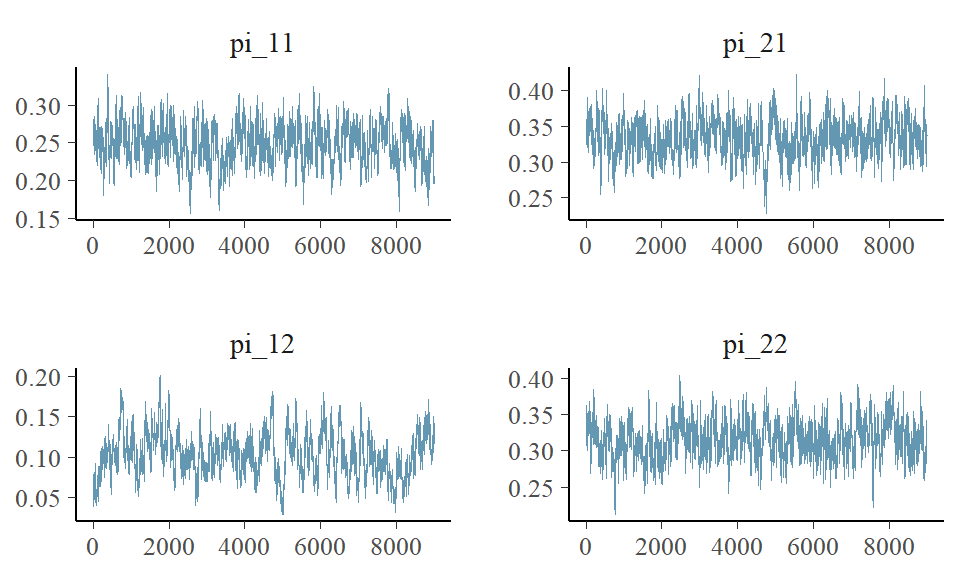
\includegraphics{dppaper_files/figure-latex/unnamed-chunk-12-1} \end{center}

log odds distribution

\begin{verbatim}
#>     2.5%      50%    97.5% 
#> 1.297400 2.289552 4.785425
\end{verbatim}

\begin{center}\includegraphics{dppaper_files/figure-latex/unnamed-chunk-13-1} \end{center}

(Insert gdp Analysis Here)

For clean data, a estimate for the odds ratio and a confidence interval
can be constructed using Woolf's method (i.e.~A wald confidence interval).
It uses the fact that the log of the odds ratio is approximately
normal for large sample sizes.
\[
\log\left(\dfrac{n_{11} \cdot n_{22}}{n_{12} \cdot n_{21}}\right) 
  \pm z_{\alpha/2}\sqrt{\dfrac{1}{n_{11}} + \dfrac{1}{n_{22}} + \dfrac{1}{n_{12}} + \dfrac{1}{n_{21}}}
\]

\begin{verbatim}
or_confint <- function(x, alpha) {
  or <- log(x[1] * x[4]/ (x[2] * x[3]))
  se <- sqrt(sum(1/x))
  c(or - qnorm(alpha/2) * se, or + qnorm(alpha/2) * se)
}

#clean data
exp(or_confint(x, .95))
\end{verbatim}

\begin{verbatim}
#> [1] 1.848471 1.833718
\end{verbatim}

\begin{verbatim}
#privitized data
exp(or_confint(sdp, .95))
\end{verbatim}

\begin{verbatim}
#> [1] 2.293115 2.274220
\end{verbatim}

\hypertarget{logistic-regression}{%
\subsection{Logistic Regression}\label{logistic-regression}}

\hypertarget{summary}{%
\section{Summary}\label{summary}}

This package is cool. You should install it.

\hypertarget{references}{%
\section*{References}\label{references}}
\addcontentsline{toc}{section}{References}

\hypertarget{refs}{}
\begin{CSLReferences}{1}{0}
\leavevmode\vadjust pre{\hypertarget{ref-Carroll2006}{}}%
Carroll, Raymond J., David Ruppert, Leonard A. Stefanski, and Ciprian M. Crainiceanu. 2006. \emph{Measurement Error in Nonlinear Models}. Chapman; Hall/CRC. \url{https://doi.org/10.1201/9781420010138}.

\leavevmode\vadjust pre{\hypertarget{ref-Dwork2013}{}}%
Dwork, Cynthia, and Aaron Roth. 2013. {``The Algorithmic Foundations of Differential Privacy.''} \emph{Foundations and Trends{\textregistered} in Theoretical Computer Science} 9 (3-4): 211--407. \url{https://doi.org/10.1561/0400000042}.

\leavevmode\vadjust pre{\hypertarget{ref-Gong2022}{}}%
Gong, Ruobin. 2022. {``Transparent Privacy Is Principled Privacy.''} \emph{Harvard Data Science Review}, no. Special Issue 2 (June). \url{https://doi.org/10.1162/99608f92.b5d3faaa}.

\leavevmode\vadjust pre{\hypertarget{ref-Ji2014}{}}%
Ji, Zhanglong, Zachary C. Lipton, and Charles Elkan. 2014. {``Differential Privacy and Machine Learning: A Survey and Review.''} \url{https://arxiv.org/abs/1412.7584}.

\leavevmode\vadjust pre{\hypertarget{ref-Ju2022}{}}%
Ju, Nianqiao, Jordan Awan, Ruobin Gong, and Vinayak Rao. 2022. {``Data Augmentation {MCMC} for Bayesian Inference from Privatized Data.''} In \emph{Advances in Neural Information Processing Systems}, edited by Alice H. Oh, Alekh Agarwal, Danielle Belgrave, and Kyunghyun Cho. \url{https://openreview.net/forum?id=tTWCQrgjuM}.

\leavevmode\vadjust pre{\hypertarget{ref-Karwa2015}{}}%
Karwa, Vishesh, Dan Kifer, and Aleksandra B. Slavković. 2015. {``Private Posterior Distributions from Variational Approximations.''} \url{https://arxiv.org/abs/1511.07896}.

\leavevmode\vadjust pre{\hypertarget{ref-Robert2004}{}}%
Robert, Christian P., and George Casella. 2004. \emph{Monte Carlo Statistical Methods}. \emph{Springer Texts in Statistics}. Springer New York. \url{https://doi.org/10.1007/978-1-4757-4145-2}.

\leavevmode\vadjust pre{\hypertarget{ref-Smith2011}{}}%
Smith, Adam. 2011. {``Privacy-Preserving Statistical Estimation with Optimal Convergence Rates.''} In \emph{Proceedings of the Forty-Third Annual ACM Symposium on Theory of Computing}. STOC'11. ACM. \url{https://doi.org/10.1145/1993636.1993743}.

\leavevmode\vadjust pre{\hypertarget{ref-Yi2017}{}}%
Yi, Grace Y. 2017. \emph{Statistical Analysis with Measurement Error or Misclassification}. \emph{Springer Series in Statistics}. Springer New York. \url{https://doi.org/10.1007/978-1-4939-6640-0}.

\end{CSLReferences}

\bibliography{RJreferences.bib}

\address{%
Jordan A. Awan\\
Purdue University\\%
Department of Statistics\\ West Lafayette, IN 47907\\
%
\url{https://www.britannica.com/animal/quokka}\\%
%
\href{mailto:jawan@purdue.edu}{\nolinkurl{jawan@purdue.edu}}%
}

\address{%
Kevin Eng\\
Rutgers University\\%
Department of Statistics\\ Piscataway, NJ 08854\\
%
\url{https://www.britannica.com/animal/quokka}\\%
%
\href{mailto:ke157@stat.rutgers.edu}{\nolinkurl{ke157@stat.rutgers.edu}}%
}

\address{%
Robin Gong\\
Rutgers University\\%
Department of Statistics\\ Piscataway, NJ 08854\\
%
\url{https://www.britannica.com/animal/quokka}\\%
%
\href{mailto:ruobin.gong@rutgers.edu}{\nolinkurl{ruobin.gong@rutgers.edu}}%
}

\address{%
Nianqiao Phyllis Ju\\
Purdue University\\%
Department of Statistics\\ West Lafayette, IN 47907\\
%
\url{https://www.britannica.com/animal/quokka}\\%
%
\href{mailto:nianqiao@purdue.edu}{\nolinkurl{nianqiao@purdue.edu}}%
}

\address{%
Vinayak A. Rao\\
Purdue University\\%
Department of Statistics\\ West Lafayette, IN 47907\\
%
\url{https://www.britannica.com/animal/quokka}\\%
%
\href{mailto:varao@purdue.edu}{\nolinkurl{varao@purdue.edu}}%
}
